\chapter{The Translation Workflow}
\label{chap:workflow}

The assistant does not translate in a single step, nor does it delegate the whole task to one autonomous language-model agent which can decide freely what to do next. Instead, the translation is carried out by a semi-deterministic \emph{workflow}: a fixed arrangement of specialized stages, each responsible for one well-defined sub-problem, connected by transitions (edges) whose direction is determined by the outcome of the previous stage/stages. This chapter describes that workflow at the level of \emph{what each stage contributes} to a correct translation and \emph{why} it is shaped the way it is.

The high-level overview of the workflow is presented in \cref{sec:workflow-overview}. A concrete example of a real workflow trace is shown visually demonstrated in \cref{fig:workflow-example}. Each pipeline stage is described in detail in \cref{sec:workflow-stages}. The architectural justification for preferring an orchestrated workflow over a free agent, together with the orchestration principles that shape the graph, is developed in \cref{sec:workflow-design}. Lastly, we define the reasoning behind using a self-repair loop in \cref{sec:design-bounds}. 

For more information, the verification guarantees the workflow enforces are the subject of \cref{chap:validation}. The wording and engineering of the individual prompts belong to \cref{chap:prompting}. The concrete artifacts behind the discussion -- the data schemas, the system prompts, the harness templates, and a full execution trace -- are reproduced in \cref{app:implementation}.

\section{High-Level View}
\label{sec:workflow-overview}

The workflow is realized as a semi-deterministic \emph{state machine}: a directed graph of nodes over a shared, typed state object, executed by the LangGraph runtime\footnote{LangGraph, a library for building stateful, multi-actor applications over language models~\cite{langgraph2024}.}~\cite{langgraph2024}. A node reads the current state, performs its task -- possibly invoking a language model or an external tool -- and returns an update that is merged back into the state; an edge then decides which node runs next. The design follows the broader move in language-model systems away from a single monolithic prompt and towards \emph{compound} systems in which reasoning and acting are interleaved across several controlled steps, of which the \emph{ReAct} paradigm~\cite{yaoReActSynergizing2023} is the primary example. The assistant adopts that interleaving but constrains it: rather than letting one agent improvise the whole control flow, the order in which generation, compilation, execution, comparison, and judgment occur is fixed in advance, so that every translation is produced and checked in the same reproducible, explainable and observable way (\cref{sec:design-agent-vs-graph}).

\Cref{fig:uom-state-machine} shows the compiled graph. Execution begins at a single entry transition and terminates in one of a small number of well-defined end states: a finalized translation, a graceful abort when the request cannot be understood, or a human (user) intervention when automated repair does not converge. The path taken between entry and exit is shaped by two factors: the \emph{scope} of the request (whether the user asked to translate a schema, a query, or both) and the \emph{outcome} of each verification stage along the way.

\newgeometry{left=3cm, right=3cm, top=3cm}
\begin{figure}[t]
\centering
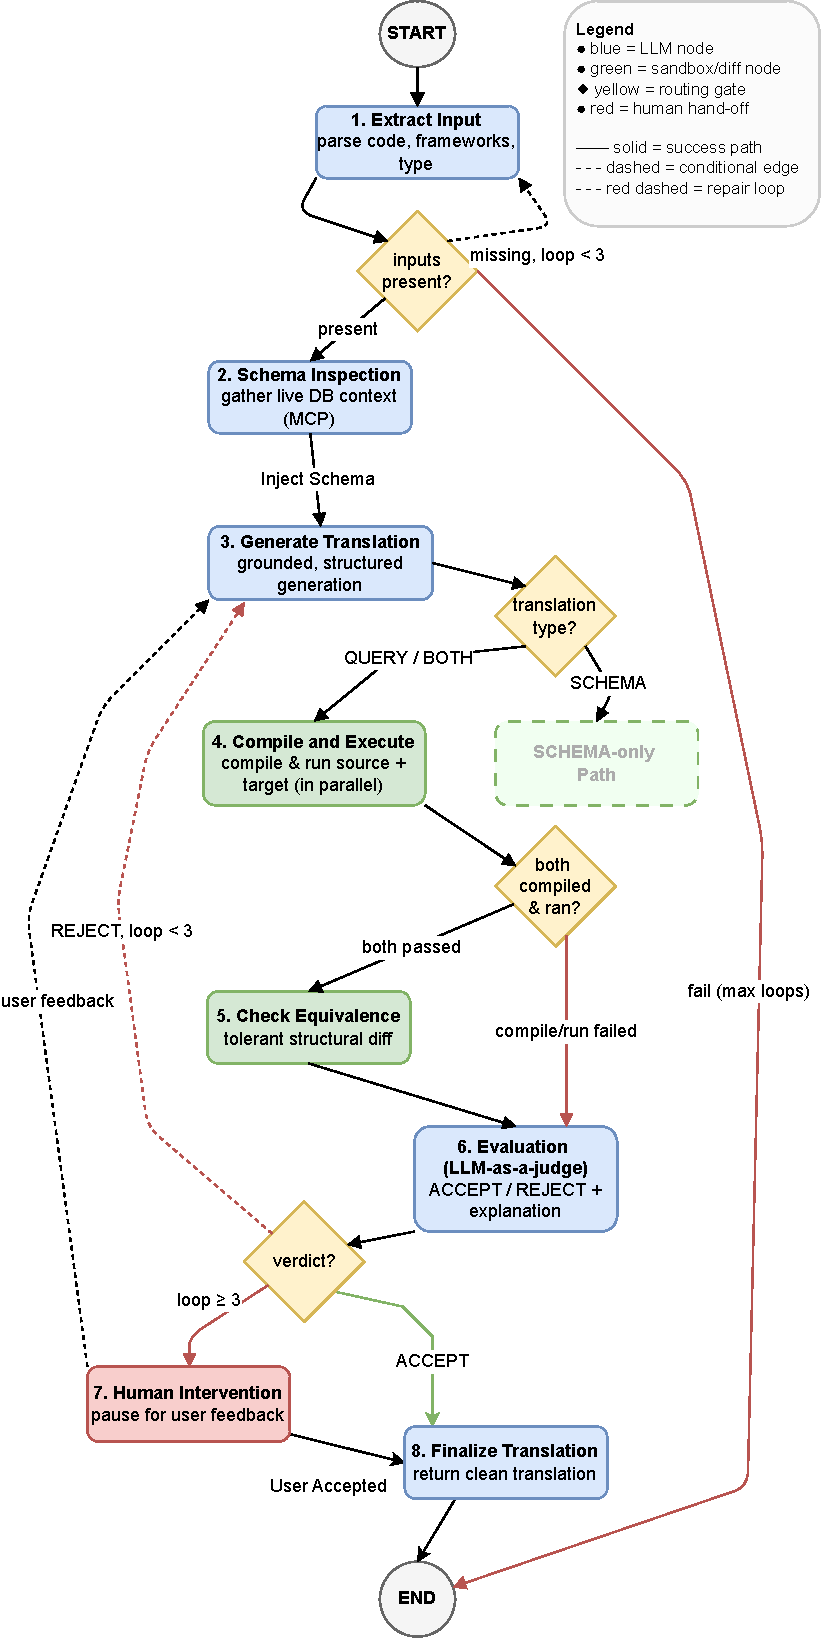
\includegraphics[width=\textwidth, height=0.9\textheight, keepaspectratio]{img/uom_state_machine.pdf}
\caption[Translation State Machine Diagram (Schema and Queries)]{State machine diagram representing the schema and query translation workflow.}
\label{fig:uom-state-machine}
\end{figure}
\restoregeometry

It is useful to distinguish three kinds of nodes, because the distinction reflects an important division of labor between the language model and deterministic code/algorithms (\cref{sec:design-state}). \emph{Generative} (blue \emph{AI} rectangles in the diagrams) nodes consult a language model to produce or judge content. \emph{Deterministic} (light blue \emph{tool calls} or purple \emph{human} rectangles) nodes contain no model call at all: they either prepare the exact inputs for a subsequent tool or execute that tool and record its result. This separation is what allows the verification steps to run in a fixed, reproducible order rather than depending on a model remembering to invoke them. \Cref{tab:workflow-nodes} lists the nodes of the graph and the default model behind each generative one.

\begin{table}[H]
\centering
\caption[The nodes of the translation workflow]{The stages of the translation workflow, classified by kind, with the default model behind each generative stage. Model names are logical aliases resolved at run time against the platform described in \cref{tab:workflow-models}; deterministic stages invoke no model.}
\label{tab:workflow-nodes}
\small
\begin{tabular}{@{}l l l@{}}
\toprule
\textbf{Stage} & \textbf{Kind} & \textbf{Default model} \\
\midrule
Input extraction        & generative & \texttt{qwen3.5-122b} \\
Schema inspection       & generative & \texttt{deepseek-v4-pro} \\
Translation generation  & generative & \texttt{kimi-k2.7-code} \\
Validation preparation  & deterministic & --- \\
Schema/query validation & deterministic & --- \\
Equivalence preparation & deterministic & --- \\
Equivalence check       & deterministic & --- \\
Evaluation (judge)      & generative & \texttt{deepseek-v4-pro} \\
Human intervention      & interrupt  & --- \\
Finalization            & generative & \texttt{kimi-k2.7-code} \\
\bottomrule
\end{tabular}
\end{table}

\subsection{The Model Portfolio}
\label{sec:workflow-models}

A single language model is not used throughout. Each stage poses a different problem -- structured output extraction, exploratory tool use, code generation, or judge verdict -- and these differ in the capabilities they reward, so the workflow assigns to each stage a model suited to it, drawing on a small portfolio of open-weight models served by the \emph{e-INFRA CZ} AI-as-a-Service platform~\cite{einfraAIaaS} through an \emph{OpenAI-compatible API}\footnote{OpenAI API Specification: https://developers.openai.com/api/reference/overview}. \Cref{tab:workflow-models} summarizes the portfolio. The selection follows two principles seen in the literature. First, strong \emph{reasoning-capable} models are used where the task is open-ended and benefits from intermediate \Acrfull{cot} reasoning -- exploratory schema inspection and code generation -- whereas a fast instruction-following non-reasoning model suffices for the near-mechanical extraction step. Second, and more importantly, the model that \emph{judges} a translation is deliberately drawn from a different family than the one that \emph{produces} it: evaluating one's own output is a known weak point of language models, and the quality of the feedback that drives repair -- rather than the act of repair itself -- has been identified as an important constraint on iterative self-correction~\cite{olaussonSelfRepair2024}. Using an independent judge mitigates the self-assessment bias documented in the LLM-as-a-judge literature~\cite{zhengJudgingLLMasaJudge2023} and is examined further in \cref{sec:validation-judge}. Lastly, the LLM leaderboards ranking by benchmark results provided by \emph{LiveBench}\footnote{\url{https://livebench.ai/}}~\cite{whiteLiveBenchChallengingContaminationLimited2025} is used to select the best-performing models for the above categories available on the \emph{e-INFRA CZ} platform at the time of writing.

\begin{table}[t]
\centering
\caption[The model portfolio]{The open-weight models behind the generative stages, served by e-INFRA~\cite{einfraAIaaS}. Parameter counts are given as \emph{total\,/\,active} for \Acrfull{moe} models where the published name discloses them; a dash denotes a figure not encoded in the released name. Quantization and context window are as configured on the serving platform. The two local fallback models are served separately through Ollama served by XRG at KSI MFF UK~\cite{xrg-mff}.}
\label{tab:workflow-models}
\small
\begin{tabularx}{\textwidth}{@{}l l l l r@{}}
\toprule
\textbf{Stage (role)} & \textbf{Model} & \textbf{Params} & \textbf{Quant.} & \textbf{Context} \\
\midrule
Generation, finalization & Qwen3.5~\cite{hfQwen35} & 397\,B / 17\,B & fp8 / int4 & $\sim$262\,k \\
Input extraction & Qwen3.5-122B~\cite{hfQwen35_122B} & 122\,B / 10\,B & fp8 & $\sim$262\,k \\
Schema inspection & DeepSeek-V4-Pro~\cite{hfDeepSeekV4Pro} & --- & fp4 & $\sim$1.05\,M \\
Evaluation (judge) & Kimi-K2.7-Code~\cite{hfKimiK27} & --- & int4 & $\sim$262\,k \\
Extraction fallback & gpt-oss-120b~\cite{hfGptOss120b} & 120\,B & mxfp4 & $\sim$131\,k \\
Local (Ollama) fallbacks & Qwen3 (27--30\,B) & 27--30\,B & --- & --- \\
\bottomrule
\end{tabularx}
\end{table}

When a stage does not specify a model, the platform default applies. Every generative stage is, moreover, backed by an ordered \emph{fallback chain} of alternative models, so that a transient outage or a persistent failure at one model escalates to the next rather than aborting the run; the principle behind these chains, and the bounded retry policy that accompanies them, is discussed in \cref{sec:design-bounds}.

\section{A Trace of a Running Example}
\label{sec:workflow-trace}

To make the abstract graph concrete, consider the running example introduced in \cref{sec:problem-example}: an Entity Framework Core (EFCore) entity together with a LINQ query, to be translated into Spring Data MongoDB. The request therefore has scope \emph{BOTH}. \Cref{tab:workflow-trace} provides a summary of the stages a concrete successful run visits, the routing decision taken after each, and the effect on the shared state. A complete, tool-level trace of the same run -- every model call and tool result, as captured by the tracing backend\footnote{Traces are captured with LangSmith and via Pydantic Logfire; see \url{https://docs.smith.langchain.com/} or \url{https://pydantic.dev/docs/logfire/get-started}.} -- is reproduced in \cref{fig:uom-trace-efcore-mongo}.

\begin{table}[H]
\centering
\caption[Execution trace of the running example]{The stages visited by a successful end-to-end run of the running example (scope \emph{BOTH}), the routing decision taken after each stage, and the resulting effect on the shared state. The same sequence is shown structurally in \cref{fig:uom-state-machine}.}
\label{tab:workflow-trace}
\small
\begin{tabularx}{\textwidth}{@{}r l X@{}}
\toprule
\textbf{\#} & \textbf{Stage} & \textbf{Routing decision and effect} \\
\midrule
1  & \emph{(entry)}            & Required inputs not yet present $\rightarrow$ extract them. \\
2  & Input extraction          & Frameworks, code, and scope identified $\rightarrow$ inputs complete. \\
3  & Schema inspection         & Source and target schemas summarized into the migration context. \\
4  & Translation generation    & Source- and target-side validation harnesses authored and saved. \\
5  & Validation preparation    & Compilation/execution of both sides requested. \\
6  & Query validation          & Both sides compiled and ran $\rightarrow$ proceed to comparison. \\
7  & Equivalence preparation    & Comparison of the two result sets requested. \\
8  & Equivalence check         & Result sets compared; differences (if any) recorded. \\
9  & Evaluation (judge)        & Evidence reviewed $\rightarrow$ \textsc{accept}. \\
10 & Finalization              & Clean target code projected from the validated harness; run ends. \\
\bottomrule
\end{tabularx}
\end{table}

A run that does not succeed on the first attempt diverges from this ideal path at a verification stage: a compilation failure, a semantic mismatch, or a rejection by the judge sends control back to translation generation with corrective feedback, and the cycle repeats under a fixed loop count before the run either succeeds or is handed to a human. A concrete example of this case is shown in \cref{fig:uom-trace-dapper-neo4j}.

\newgeometry{margin=3cm}
\begin{figure}[t]
\centering
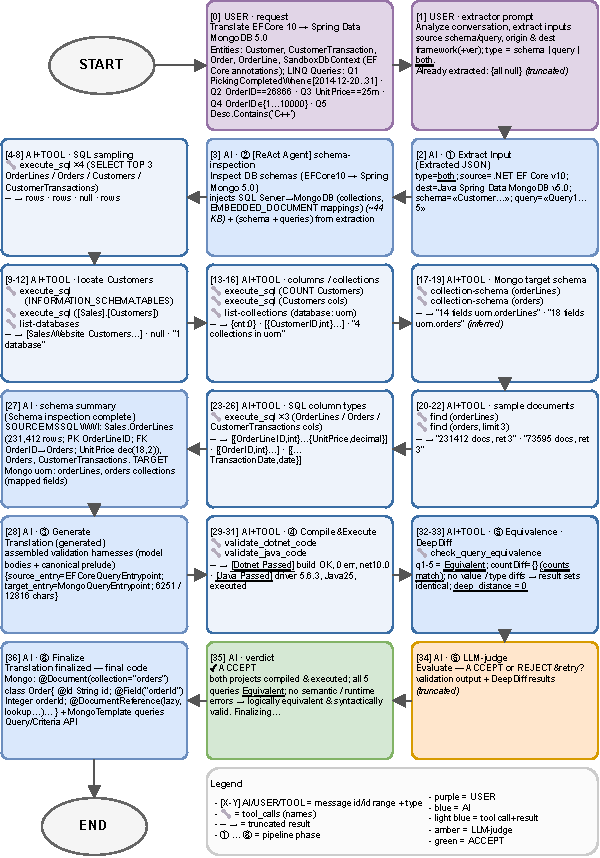
\includegraphics[width=\textwidth, height=0.9\textheight, keepaspectratio]{img/uom_trace_efcore_mongo.pdf}
\caption[EFCore to Spring Data MongoDB Translation Trace]{A complete trace of a successful end-to-end run of EFCore to Spring Data MongoDB successfully translated at first attempt. The trace shows the feedback loop in action: the first attempt succeeds, so no repair is needed.}
\label{fig:uom-trace-efcore-mongo}
\end{figure}
\restoregeometry

\newgeometry{margin=3cm}
\begin{figure}[t]
\centering
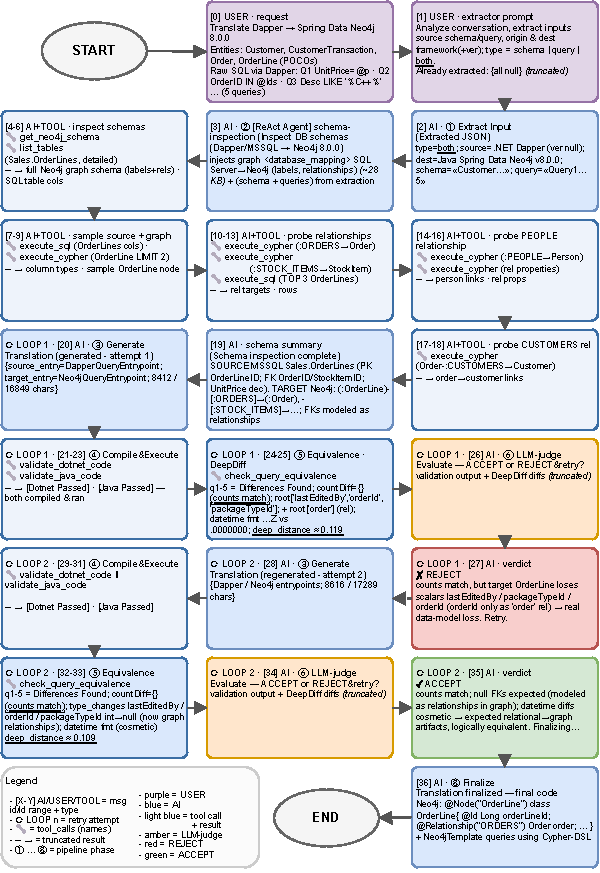
\includegraphics[width=\textwidth, height=0.9\textheight, keepaspectratio]{img/uom_trace_dapper_neo4j.pdf}
\caption[Dapper to Spring Data Neo4j Translation Trace]{A complete trace of a successful end-to-end run of Dapper to Neo4j successfully translated at second attempt, with an equivalence failure on the first. The trace shows the feedback loop in action: the first attempt fails in equivalence checking, the judge rejects it, and the second attempt succeeds.}
\label{fig:uom-trace-dapper-neo4j}
\end{figure}
\restoregeometry

\section{The Stages in Detail}
\label{sec:workflow-steps}

Each subsection below describes one stage in terms of its purpose, what it consumes and produces, the role of the language model where one is involved, and the principle that motivates its design. The full data schemas and prompts are deferred to \cref{app:pydantic-schemas,app:system-prompts}.

\subsection{Input Extraction}
\label{sec:workflow-extract}

The workflow must begin from a precise, typed description of the task, but the user expresses that task in free-form conversation\footnote{Also a structured input is possible, which skips the extraction stage, that is mainly used by \acrshort{mcp} tool input if used with other Copilots. See \cref{chap:input}.}. The first stage bridges this gap: it reads the conversation and recovers the structured parameters the rest of the pipeline depends on -- the source and target frameworks (and, if mentioned, their versions), the scope of the request (schema, query, or both), and the raw source code to be translated. This is mainly a classification-and-extraction problem rather than a reasoning one, which is why it is entrusted to a fast instruction-following model rather than a reasoning model. The model returns its answer as a typed object rather than as markdown/free-text output, so that the result can be validated mechanically against an expected shape before the workflow proceeds; the schema is reproduced in \cref{app:pydantic-schemas}. The code is captured line by line so that the original indentation -- significant in the source languages and easy for a model to corrupt -- is preserved exactly. And a dedicated \texttt{error} field lets the model report, as data, that the request cannot be fulfilled (for instance, that no translatable code was supplied), allowing the workflow to terminate cleanly with an explanation rather than proceeding on malformed input.

Extraction is robust by construction. If the model returns nothing usable, or an object still missing the minimum required fields, the stage is retried; after a fixed number (i.e. three) of unsuccessful attempts the run ends gracefully rather than looping indefinitely. This bounded-retry discipline, shared by every loop in the graph, is the mechanism by which the system honors the robustness requirement \ref{desc:requirements-r3}.

\subsection{Schema Inspection}
\label{sec:workflow-inspect}

Before any code is generated, the assistant examines the \emph{actual} databases involved in the migration. \Acrshort{llm} is asked to translate a persistence layer in the abstract will easily invent wrong collection names, field types, or relationship cardinalities. That's why grounding generation in live database schema is the established protection against such hallucination, and is the first of the verification layers set out in \cref{sec:validation-grounding}. This stage connects to the live source and target databases, inspect the schema or the entities relevant to the code at hand using specialized tools, and outputs them into a compact textual summary that is later supplied to the translation stage as part of its context (\cref{sec:prompting-context}).

The database connections are not bespoke integrations but are exposed through the \Acrfull{mcp}\footnote{The Model Context Protocol, an open standard for connecting language-model applications to external tools and data sources~\cite{modelContextProtocol2024}.}~\cite{modelContextProtocol2024}, the same open standard the project uses for all external tool access. Because inspecting a large schema is open-ended and may require many successive queries, the stage is entrusted to a reasoning-capable model and is given a mechanism to keep only the most recent observations in its working context, so that inspecting a large database does not overflow the context window (also discussed in \cref{sec:design-isolation}). Should the databases be unreachable, the stage degrades gracefully: it records that inspection was skipped and the workflow continues without a schema summary rather than failing.

\subsection{Translation Generation}
\label{sec:workflow-generate}

This is the stage where the translation is actually produced, and for that reason, it uses deliberate step-by-step generation process, which is the longest, most expensive and important stage in the pipeline. For those reasons, it runs the strongest reasoning model in the portfolio. It consumes the framework names, the scope, the source code, and the schema summary, and it is supplied with a system prompt assembled specifically for the framework pair at hand -- carrying the translation contract, the framework-specific rules, the exact pinned dependency versions, and worked structural examples. The construction of that prompt is the subject of \cref{sec:prompting-grounding}.

A design decision made here propagates through the rest of the workflow: this stage does \emph{not} emit the polished, user-facing translation. Instead it authors the material needed to \emph{verify} a translation -- runnable harnesses for the source and target sides -- and defers production of the clean answer until after that material has passed every check (\cref{sec:workflow-finalize}). The published result is thus never an unverified claim by the model but always a projection of code that has demonstrably compiled, executed, and preserved the query's meaning. This reflects the principle, established in execution-based evaluation of generated code, that correctness should be decided by running the code rather than by inspecting it~\cite{chen2021codex,execoder2025}.

The stage operates as a tool-calling agent in the ReAct style~\cite{yaoReActSynergizing2023}: it may consult documentation and the web to get an unfamiliar \acrshort{api} right before committing,\footnote{Documentation search is provided through the Spring and Microsoft documentation services exposed over \acrshort{mcp}; open-web search uses the Tavily API, \url{https://www.tavily.com/}.} and it concludes by recording its result through a series of dedicated \emph{save tools}. Notably, it is \emph{not} given the database-inspection tools (the schema was already summarized upstream) nor the validators (verification is performed by the dedicated downstream stages); restricting the tool surface keeps the agent focused on generation and prevents it from exhausting its maximum step count in redundant exploration, a known problem of ReAct agents being exposed to many redundant tools. Only the genuinely variable part of the code is authored by the model; the unchanging scaffolding on which the validators depend is supplied deterministically, a separation explained in \cref{sec:prompting-context} and reproduced in \cref{app:snippets}. The generation schema and the finishing action are documented in \cref{app:pydantic-schemas}.

\subsection{Compilation and Execution}
\label{sec:workflow-validate}

Producing syntactically plausible code is not the same as producing code that builds and runs, and the gap between the two is exactly where \acrshort{llm} code generation fails -- through hallucinated APIs, missing dependencies, or type errors~\cite{spracklenPackageHallucinations2025}. The workflow therefore compiles and executes both the source and the target translations against real \acrshort{cli} tools and databases. This is carried out by two deterministic stages: a preparation stage assembles the precise validation request, and an execution stage runs it. Splitting the work this way -- rather than trusting the generative model to remember to compile its own output -- is what makes the order and the content of verification reproducible.

For a schema-only request, only the translated entities are compiled\footnote{Path not shown in \cref{fig:uom-state-machine}; but is structurally very similar to it}. For a request involving queries, both sides are compiled \emph{and} executed, and -- because the two sides are independent -- they are processed in parallel. Each side is built and run inside an isolated, disposable sandbox provisioned for the purpose\footnote{Sandboxes are provisioned and executed through a self-deployed Daytona instance~\cite{daytona2026}.}~\cite{daytona2026}; the execution writes its query results out in a normalized form that the next stage can compare. The full mechanics of the sandboxes -- how projects are assembled, how files are transported, and how build output is captured -- are described in \cref{sec:validation-sandbox}. What matters at the level of the workflow is the contract: each side reports whether it compiled and ran, and a failure here does not abort the run but is fed back to the generation stage for correction.

\subsection{Equivalence Checking}
\label{sec:workflow-equivalence}

Compilation establishes that a translation is well-formed; it says nothing about whether the translated query \emph{returns the same data} as the original. Establishing that is the role of the equivalence check, reached only once both sides have executed successfully. It compares the result sets the two sides produced -- their row counts and representative sample records -- and records any differences for the downstream judge and for any subsequent repair attempt. The comparison is deliberately tolerant of differences that are provably immaterial to meaning, such as field ordering, harmless numeric-precision variation, or a reversed sort order, in keeping with the semantic preservation requirement \ref{desc:requirements-r2}. Comparing \emph{observed execution results} rather than the code itself is what makes the check a genuine test of semantic equivalence rather than of surface similarity, echoing the executability-oriented approach to code translation~\cite{execoder2025}. The comparison is computed with the DeepDiff library\footnote{DeepDiff, a structural difference engine for Python objects~\cite{deepdiff}.}~\cite{deepdiff}; because its algorithm, its tolerance rules, and the serialisation contract that makes the two result sets comparable are central to the correctness argument of this thesis, they are treated in full in \cref{sec:validation-equivalence} rather than here.

\subsection{Evaluation: \Acrshort{llm}-as-a-Judge}
\label{sec:workflow-judge}

The equivalence check produces evidence -- compiler outcomes and a structural diff of the results -- but evidence still has to be interpreted: a recorded difference may be a harmless artifact or a genuine semantic error. The workflow resolves this with an independent language model acting as a judge, a now-standard technique for automated quality assessment whose strengths and biases are characterized by Zheng et al.~\cite{zhengJudgingLLMasaJudge2023}. The judge reads the accumulated evidence and returns a binary verdict -- accept or reject -- together with a justification reasoning. The verdict decides whether the run proceeds to finalization or returns for another attempt.

Two design choices follow directly from the literature. The judge is required to supply a justification, never a bare verdict, both for observability and because the written reasoning is the repair signal\footnote{This could imagined as an instance of the Tree-of-Thought (ToT) thinking process~\cite{yaoTreeThoughtsDeliberate2023}}~\cite{yaoTreeThoughtsDeliberate2023} -- and the usefulness of that signal, not the repair mechanism, is what controls whether iterative correction succeeds~\cite{olaussonSelfRepair2024}. And the judge runs a different model from the generator, so that the system does not grade its own work; the judge's role is to interpret deterministic evidence, not to reframe correctness, which keeps its authority bounded and is the basis of the trust argument in \cref{sec:validation-judge}.

\subsection{Human Intervention}
\label{sec:workflow-human}

Automated self-repair is powerful but not unconditionally reliable; the empirical finding that it is \emph{"not a silver bullet"}~\cite{olaussonSelfRepair2024} is taken seriously in the design. When repeated automated attempts fail to converge, or when the generator cannot produce well-formed output at all, the workflow does not loop indefinitely or emit a hallucinated result. It pauses and hands control to a human reviewer, showing the current state -- the validated artifacts produced so far, the judge's explanation, the recorded differences, and the entire chat conversation with intermediate results -- for inspection. The reviewer either accepts the current translation, sending the run to finalization, or rejects it with feedback, which re-enters the repair cycle exactly as an automated rejection would. This controlled hand-off is the graceful-degradation half of requirement \ref{desc:requirements-r3}, and the fraction of runs that reach it is another metric requirement \ref{desc:requirements-r4} that the evaluation reports (\cref{chap:evaluation}).

\subsection{Finalization}
\label{sec:workflow-finalize}

The last stage runs only after a translation has been accepted -- by the judge, by a clean compilation in the schema-only case, or by a human reviewer. Its task is not to translate but to \emph{extract}: it takes the already-validated harness, which is the authoritative source of truth, and projects from it the clean, production-ready target code the user will see, stripping away the scaffolding that existed only for verification while preserving every annotation and predicate that the checks confirmed. Because its input is fixed once validation has passed, finalization is a constrained projection rather than a fresh generation, which guarantees that the published answer is always a faithful rendering of verified code.

Separating finalization from generation serves a second purpose specific to the evaluation. Because the published code is the artifact compared across experimental runs by a structural code-similarity metric (\cref{chap:evaluation}), it must be produced under fixed conditions: this stage therefore pins one specific model with no fallback and temperature set to zero.

\section{Design Rationale and Orchestration}
\label{sec:workflow-design}

The shape of the workflow is the outcome of a sequence of design decisions, several of which reversed an earlier, more autonomous prototype of the assistant. This follows the distinction, now standard in the engineering literature on language-model systems, between a \emph{workflow} -- a system in which models and tools are orchestrated along predefined code paths -- and an \emph{agent} -- a system in which the model dynamically directs its own process and tool usage~\cite{anthropicBuildingEffectiveAgents2024}. The \cref{sec:design-agent-vs-graph}, \cref{sec:design-state}, \cref{sec:design-isolation}, and \cref{sec:design-bounds} below explain the rationale behind the current state of the workflow design, and how we got to it.

\subsection{A Free ReAct Agent versus an Orchestrated Graph}
\label{sec:design-agent-vs-graph}

The first prototype of the assistant was a single ReAct agent~\cite{yaoReActSynergizing2023}: one reasoning model equipped with every tool the task could need -- database inspection, documentation search, both compilers, and the equivalence checker -- and instructed to translate, validate, and finish with one structured answer. This design is attractive on paper because the model decides for itself when to inspect, generate, and verify. In practice, it showed exactly the failures that the engineering literature attributes to premature agentic autonomy~\cite{anthropicBuildingEffectiveAgents2024}. The agent would skip or reorder verification steps, since nothing but the prompt compelled it to compile its own output; it would burn its maximum step count on redundant database exploration and reach the recursion limit before saving a result; the verbose compiler and diff output it pulled into its own context degraded subsequent generation; and, because every run improvised a different tool sequence, no two runs were comparable, which made systematic evaluation impossible.

The production design switches the responsibility. The \emph{order} of generation, compilation, execution, comparison, and judgment is fixed by the graph's edges and cannot be skipped or rearranged by any model. The model's autonomy is spread into individual, self-contained stages, where it is genuinely useful -- deciding which documentation to consult before generating, or which entities to inspect in a large schema. Each such inner agent, or \emph{subagent}\footnote{In LangGraph terms also referred to as \emph{subgraph}}, runs with a deliberately restricted tool choices (\cref{sec:workflow-generate}) and a bounded step count. The result is a \emph{semi-deterministic} system: creative where creativity is required (temperature unchanged), deterministic everywhere correctness is compulsory. This is what makes every run observable, explainable, reproducible in structure, and directly comparable in the evaluation (\cref{chap:evaluation}).

\subsection{Typed Shared State and Stateless Nodes}
\label{sec:design-state}

The stages communicate exclusively through a single shared state object: a typed record whose fields carry the extracted inputs, the schema summary, the generated harnesses, the validation results, the equivalence diffs, and the loop counters. A node is a pure function of this state -- it reads what it needs, performs its task, and returns a partial update that the runtime merges back. The LangGraph graph is implemented using Google's Pregel ecosystem~\cite{google-pregel}: a robust system for large-scale graph processing, specifically tailored for low-level \acrshort{llm} orchestration. Because the complete state is externalized, the runtime can checkpoint it at every transition, which is what allows a run to pause indefinitely at the human-intervention stage and resume later without loss (\cref{sec:workflow-human}). Because nodes are stateless, each can be independently retried on transient failure, cached when its inputs have not changed, and observed in isolation by the tracing backend (LangSmith or LogFire). And because the state is typed, the contract between stages is machine-checked rather than implied: a stage cannot silently consume a field that no upstream stage produces. The state purposefuly distinguishes a narrow \emph{Input} interface (what a user must supply) and a narrow \emph{Output} interface (what a user receives back) from the wider internal \emph{State}, so the graph presents a stable API surface to the surrounding application (\cref{chap:architecture}).

\subsection{Keeping the Reasoning Context Clean}
\label{sec:design-isolation}

\Acrshort{llm}s degrade measurably as their input context grows and as relevant information is buried among irrelevant text~\cite{liuLostInTheMiddle2024}; managing what enters a model's context is therefore an engineering concern of the same rank as prompt wording~\cite{anthropicContextEngineering2025}. Four mechanisms allow this to be done systematically.

First, huge intermediate artifacts live in dedicated state fields, not in the conversational history: the schema summary, the harness code, and the equivalence diffs are stored as data and injected into a prompt only where and when they are needed. Second, the verification loop runs on a message channel separate from the user-facing (UI) conversation, so that iterative trial-and-error logs never pollute the primary thread. Third, the interior agents apply context editing: the schema-inspection agent, which may issue dozens of database queries, retains only its most recent tool results once a token threshold is exceeded, and the generation agent summarizes its own history if it approaches its context limit. Fourth, a failed attempt is never replayed verbatim into the next one; instead, the failure signals -- the judge's explanation, the last few tool outputs, and the diffs -- are \emph{distilled} into a compact textual note. The distillation additionally neutralizes bare verdict tokens such as \textsc{rejected} in the quoted feedback, because a low-temperature model shown such an attentive token (i.e. \emph{ACCEPT}/\emph{REJECT}) can copy it verbatim into a code field -- a degenerate failure observed in practice.

\subsection{Bounded Loops, Retries, and Fallbacks}
\label{sec:design-bounds}

\Acrshort{llm} code generation fails in characteristic ways -- invented APIs, type mismatches, malformed structured output~\cite{spracklenPackageHallucinations2025}. The workflow mitigates them through four nested layers, each bounded by a small constant, ordered from the innermost outward. At the innermost layer, a model whose structured response fails schema validation is re-invoked \emph{in place} with a concise description of exactly what was wrong. At the second layer, every external tool invocation -- sandbox provisioning, compilation, the equivalence check -- is retried with exponential backoff against transient infrastructure errors, and a terminal tool failure is converted into a structured failure message, so the run continues and the failure becomes repair feedback. At the third layer, each generative stage carries an ordered \emph{fallback chain} of alternative models: a model that is unavailable or persistently erroring is replaced by the next entry, ending at a locally served model that keeps the assistant alive even if the last models are not that performant. At the outermost layer there are the loop thresholds already described: a fixed number of extraction attempts and a fixed number of translation-repair attempts.

The stages described above are connected so that every verification failure feeds back into a new generation attempt, making the workflow a \emph{self-repairing} system in the sense of Chen et al.~\cite{chenSelfDebug2023}: rather than discarding a failed attempt, the model is shown the consequences of its output -- compiler diagnostics, the equivalence diff, the judge's critique -- and asked to repair itself. Execution feedback of this kind has been shown to improve generated-code accuracy substantially over single-shot generation~\cite{chenSelfDebug2023}.
